	\chapter{Computer Vision Prework}

	\section{Emergence of Convolution}
	\subsection{Feature Extraction}
	\begin{bulletedlist}
		\item What is a feature (in an image)?
		\begin{bulletedlist}
			\item Features are various forms of information that can be gained from an image.  For example: Fig 1 has various features, such as shape, size, color, edges, and background.  These features play a crucial role in helping perform several tasks in computer vision like image classification, object detection, scene detection, etc.
		\end{bulletedlist}
		\item The features required by each task in computer vision are completely task-dependent, and each task might not require all the features available in an image.  For example, we can still identify that the right side of \figurename~\ref{fig:imagefeatureextraction} is an image of a duck (even though it is harder to do than for the left) without necessarily knowing the color or background of the image, but only from looking at the edges, the presence of water and the shape of the bird inside the image.
		\item Hence, we need methods to extract just the essential information contained in images and ignore the rest depending on different tasks. This step is called feature extraction.
		\item The features we obtain from feature extraction are crucial in enhancing the model's performance.
		\item Feature extraction methods help in converting images to certain feature vectors of fixed sizes.
		\item Some of the most important feature extraction techniques to have been used with images are:
		\begin{bulletedlist}
			\item HOG (Histogram of Oriented Gradients)
			\item SIFT (Scale Invariant Feature Transform)
			\item Convolution Operations
		\end{bulletedlist}
	\end{bulletedlist}

	\begin{figure}[h]
		\centering
		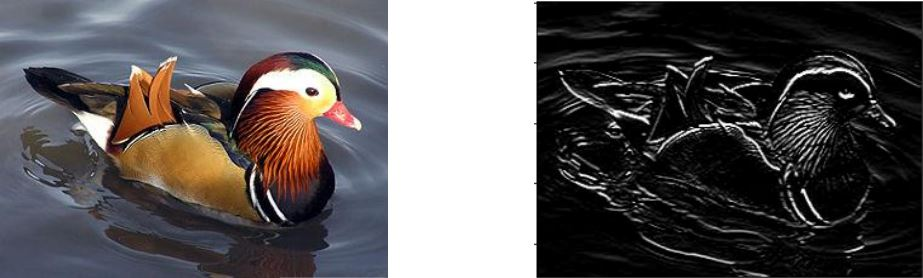
\includegraphics[height=1.5in]{imagefeatureextraction}
		\caption{Feature extraction.}
		\label{fig:imagefeatureextraction}
	\end{figure}

	\subsection{Conventional Feature Extraction Techniques}
The two most historically-important, manual feature extraction techniques have been:
	\begin{bulletedlist}
		\item HOG (Histogram of Oriented Gradients)
		\item SIFT (Scale Invariant Feature Transform)
	\end{bulletedlist}

	\begin{table}
		\begin{tabular}{|p{0.5\textwidth-2\tabcolsep}|p{0.5\textwidth-2\tabcolsep}|} \hline
				\tablecolumnheadervlinesone{HOG} & \tablecolumnheadervlinestwo{SIFT} \\ \hline
				HOG mainly focuses on the structure and shape of an object. &
	            In SIFT, image content is converted into local feature coordinates that are not affected by rotation, scaling, or other
	image manipulations. \\ \hline
				HOG is different from only detecting edges, as it also identifies the magnitude and direction of edges in the image. &
	            SIFT assists in locating the local features of an image, often known as image keypoints. \\ \hline
				HOG calculates the magnitude and direction of edges in each region. The Orientation is the direction and the Gradient is the magnitude of the pixel values of the image. &
				The key points obtained from SIFT can be utilised for picture matching, object detection, scene detection, and other computer vision applications. \\ \hline
				\adjustbox{center}{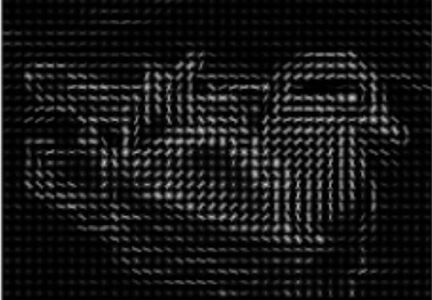
\includegraphics[height=1.5in]{hogfeaturedetection}} &
				\adjustbox{center}{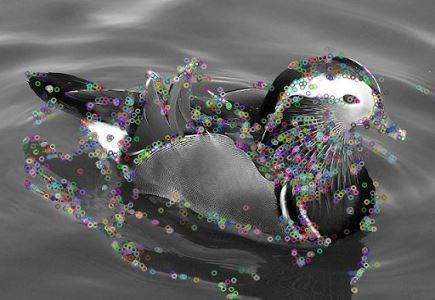
\includegraphics[height=1.5in]{siftfeaturedetection}} \\ \hline
		\end{tabular}
	\end{table}

	\subsection{Disadvantages of Conventional Feature Extraction Techniques}
	\begin{bulletedlist}
		\item Why was SIFT preferred over HOG?
		\begin{bulletedlist}
			\item SIFT features, as opposed to HOG features, have the advantage of being unaffected by the image's size or orientation.
			\item SIFT has a better accuracy than HOG for detecting features in an image.
			\item HOG is not scale and rotation invariant, whereas SIFT shows those properties.
		\end{bulletedlist}
		\item However, both SIFT and HOG showed certain disadvantages in the efforts to apply them as general feature extraction techniques for all images:
		\begin{bulletedlist}
			\item Both SIFT and HOG are quite slow and computationally expensive.
			\item They are also somewhat mathematically complex in their working.
			\item In addition, HOG does not work well with lighting changes and blurring in the images.
		\end{bulletedlist}
	\end{bulletedlist}

	\subsection{Convolution Over SIFT and HOG}

	\begin{bulletedlist}
		\item Convolution is a specialized linear operation on an image, that represents an efficient way of extracting image features and reducing the dimensions of an image.
		\item Convolution consists of a set of filters called convolution layers, that perform convolution operations on images.
		\item We use multiple filters to perform convolution operations on an image, and try to extract various kinds of features (pertaining to each kind of filter) from a single image.
		\item For example, let's assume that we need to use convolutions to extract features from an image of a brick wall (shown in \figurename~\ref{fig:convolutionbrickwall}).  We may be interested in each of the following feature extraction tasks:
		\begin{bulletedlist}
			\item to extract all the vertical edges from the image
			\item to extract all the horizontal edges from the image
			\item to blur/sharpen the image
			\item To highlight/focus on certain places of image
		\end{bulletedlist}
		\item As seen from the below example in \figurename~\ref{fig:convolutionbrickwalledgedetection}, convolution filters can help us achieve any of the feature extraction tasks we may require for our images.
	\end{bulletedlist}


	\begin{figure}[h]
		\centering
		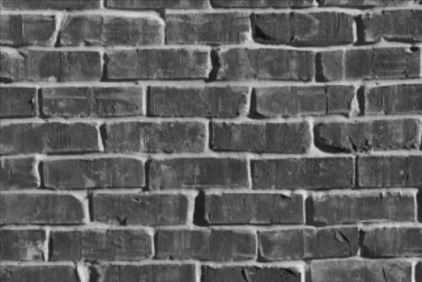
\includegraphics[height=1.5in]{convolutionbrickwall}
		\caption{Image of a brick used for convolution example.}
		\label{fig:convolutionbrickwall}
	\end{figure}

	\begin{figure}[h]
		\centering
		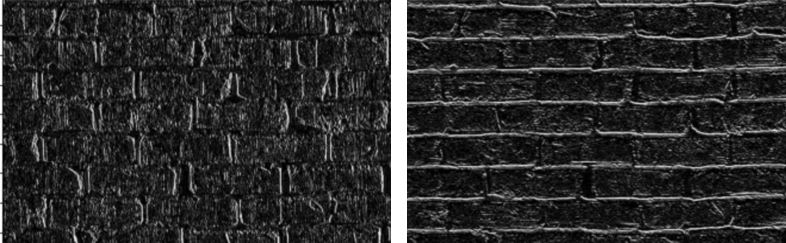
\includegraphics[height=1.5in]{convolutionbrickwalledgedetection}
		\caption{Image of brick wall with vertical edge detection (left) and horizontal edge detection (right).}
		\label{fig:convolutionbrickwalledgedetection}
	\end{figure}

	\subsection{Convolution over SIFT and HOG}

Why is Convolution better than SIFT and HOG?
	\begin{bulletedlist}
		\item Convolutional feature detectors are highly trainable and adaptable, allowing them to achieve higher accuracy levels in comparison to SIFT and HOG for the task at hand.
		\item Convolutions excel at learning low-level features of an image in a much better way than SIFT and HOG, and they do so without the overhead of the hand-coded feature engineering which is usually required for SIFT and HOG.
		\item Apart from learning low-level features, hierarchical combinations of convolutions are quite effective in learning important high-level features as well.  Example: for images of human faces, convolutional layers would easily learn to understand more
complex shapes such as the eyes, the ears, the nose or the mouth.
		\item In 2012, AlexNet, a Convolutional Neural Network (CNN) architecture, based fundamentally on the principle of convolutional filters, handily won the famous ImageNet competition - outperforming the runner-up by over 10 percentage points.  Although convolutions were already known in literature from the work of Yann LeCun, this breakthrough is what drew attention from the whole technology industry to the power of convolutions in image feature extraction.
		\item It soon became clear to machine learning practitioners that hierarchical combinations of convolution filters achieved superior and far more generalizable results in image feature extraction than SIFT and HOG. This is the fundamental driver behind the emergence of convolutions as part of Convolutional Neural Networks (CNNs), which have become a staple in state-of-the-art deep learning models for computer vision over the last decade.
	\end{bulletedlist}



	\section{Edge Detection and Kernels}
	\subsection{Convolution and Edge Detection}
	\subsubsection{Edge Detection}
	\begin{bulletedlist}
		\item As we previously discussed, the Convolution operation is the fundamental building block of Convolutional Neural Networks.

		\item Let's try to understand how the Convolution process works, with the help of the Edge Detection concept that Convolution filters are able to perform.
		\item Mathematically in terms of pixel intensity values, edges are image regions where there is a sudden, sharp change in the brightness of the pixels. This can be observed by a large change in the pixel intensity values among neighboring pixels in some direction.
		\item Let us first convert the image in \figurename~\ref{fig:edgedetectioncross} into its gray scale version, so that we have a 2D matrix to work with for us to analyze the pixel intensity values of the image (\figurename~\ref{fig:convolutionbrickwalledgedetection}).
		\item The information about edges in images is usually preserved during gray scale conversion for most of the images we will work with, so we don't have to worry about color information loss for now.
		\item We observe that there is a clear gradient or change in pixel intensity values either side of the lines drawn inside this matrix. (Ex: 255 on one side and 116 and 61 on the other).
		\item These gradient lines also mirror the ``+'' shape of the edges of the image, so we know that they are a mathematical representation of what we visually perceive to be edges inside the image.
		\item This gradient of pixel intensity values is hence the mathematical meaning of an edge inside an image.
		\begin{bulletedlist}
			\item
		\end{bulletedlist}
	\end{bulletedlist}

	\begin{figure}[h]
		\centering
		
\includegraphics[height=1.0in]{edgedetectioncross}
		\caption{}
		\label{fig:edgedetectioncross}
	\end{figure}
	\begin{figure}[h]
		\centering
		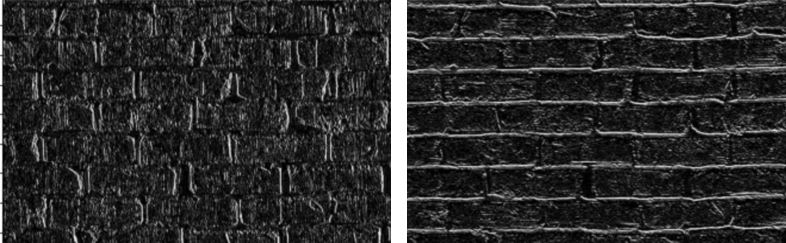
\includegraphics[height=1.5in]{convolutionbrickwalledgedetection}
		\caption{}
		\label{fig:convolutionbrickwalledgedetection}
	\end{figure}
	\begin{figure}[h]
		\centering
		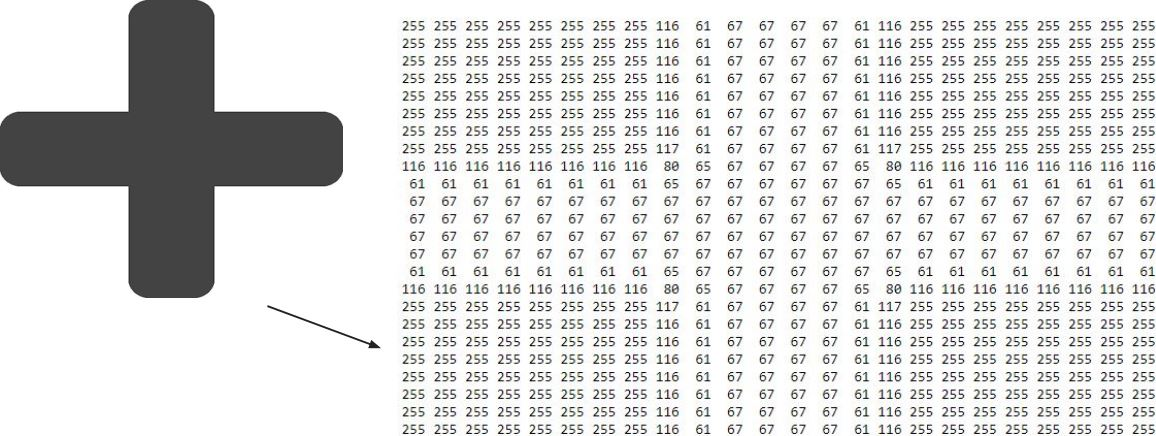
\includegraphics[height=1.5in]{edgedetectioncrossgrayscale}
		\caption{}
		\label{fig:edgedetectioncrossgrayscale}
	\end{figure}
	\begin{figure}[h]
		\centering
		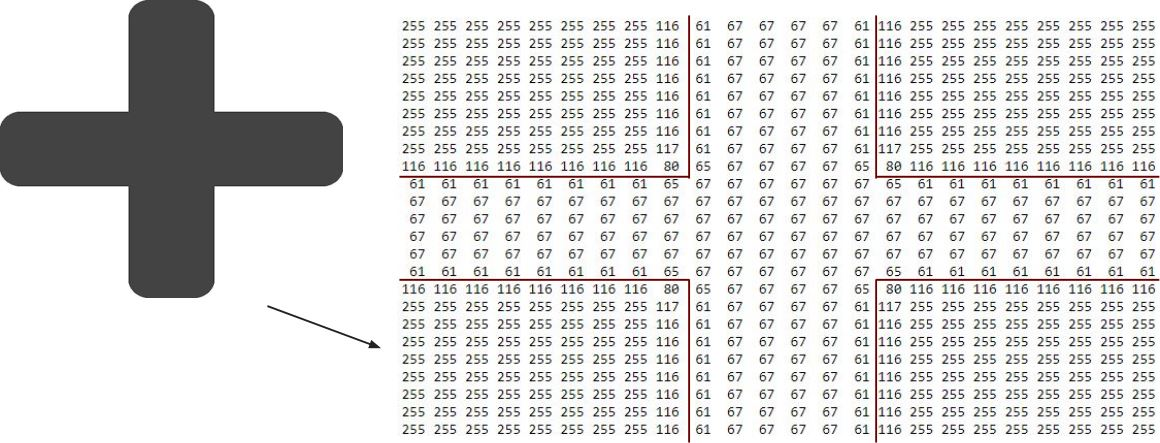
\includegraphics[height=1.5in]{edgedetectioncrossgrayscale2}
		\caption{}
		\label{fig:edgedetectioncrossgrayscale2}
	\end{figure}

	\subsection{The importance of Edges}
	\begin{bulletedlist}
		\item So why are edges important?  Let's try to understand this with an example.
		\item In the left side of \figurename~\ref{fig:edgedetectioncar}, we have a gray scale image of a Ferrari 456 GT, a famous sports car from the nineties.
		\item On the right is another version of the same image, but with purely the edges of the image of the car on the left, and with very little information retained about the background.
		\item Can we still identify the presence of the car despite this loss of information?  Yes, we can!
		\item What this means, is that we can identify objects in an image based purely on the information about their edges, even by completely ignoring their background or other minute details of the image that are not important in detecting that object.
Therein lies the importance of edges in image prediction tasks.
		\item Edge detection is one of the primary tasks in object detection and object recognition.
		\item A lot of information about an image is found within its edges. So detecting edges and enhancing those areas should be our focus in image processing for the purpose of image classification tasks.
		\item One way to mathematically detect edges in an image is to perform convolution operations on a input image with a small array of numbers, also called a Filter / Kernel.
		\item The term Kernel refers to a 2D array, while the term Filter generally refers to multiple kernels stacked
together, to operate across a whole N-dimensional array. However the terms Kernel and Filter are often
used interchangeably across the industry.
		\item There are essentially three steps involved in the convolution operation:
		\begin{numberedlist}
			\item Taking in the Input Image as a Pixelmap.
			\item Applying a Filter / Kernel on the Input Image Pixelmap.
			\item Obtaining the Output Feature map
		\end{numberedlist}
	\end{bulletedlist}

	\begin{figure}[h]
		\centering
		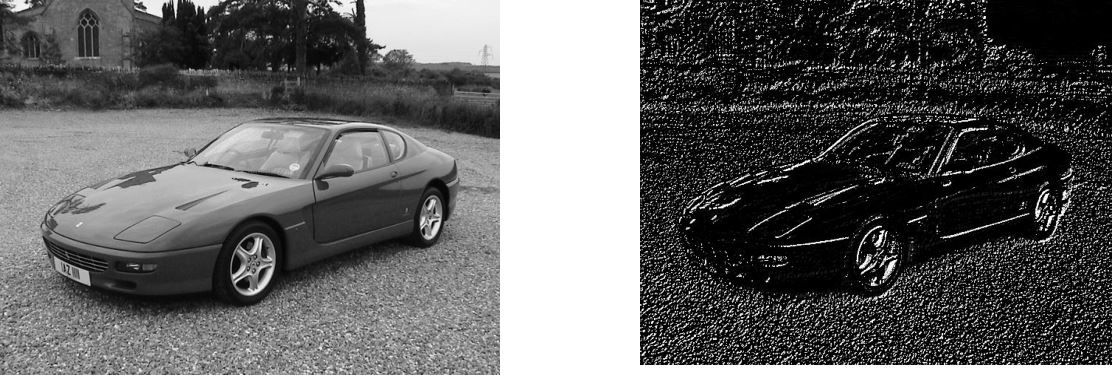
\includegraphics[height=1.5in]{edgedetectioncar}
		\caption{}
		\label{fig:edgedetectioncar}
	\end{figure}

	\subsection{How to Detect Edges}

	\begin{bulletedlist}
		\item \figurename~\ref{fig:convolutededgedetection} is a representation of this three-stage convolution process.
		\item In the process, an input image (taken in the form of its pixelmap) is convolved with a kernel or filter, 	in order to obtain an output feature map.
		\item The above filter containing 1s, 0s and -1s, is an example of a vertical edge detector, as the pattern of numbers in the filter is vertically consistent (top to bottom) and will hence likely detect vertical edges inside the image.
		\item Let us now try to understand the mathematical working of convolution kernels, in order to understand the intuition behind how kernel edge detectors work.
	\end{bulletedlist}

	\begin{figure}[h]
		\centering
		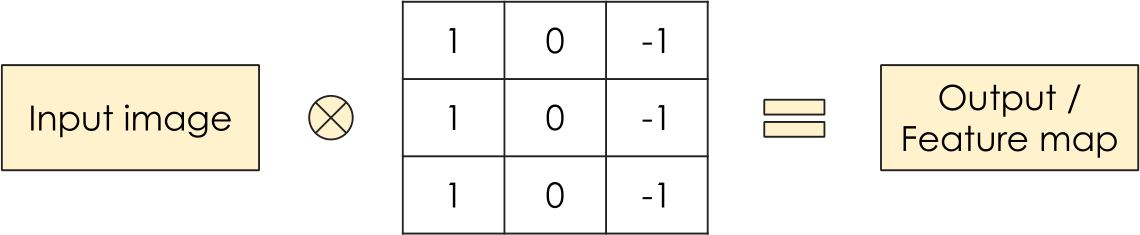
\includegraphics[height=1.25in]{convolutededgedetection}
		\caption{}
		\label{fig:convolutededgedetection}
	\end{figure}

	\begin{numberedlist}
		\item The filter is first superimposed over the first corresponding 3 x 3 region of the image, taking the products of the corresponding elements from the image and the filter, and then adding all these products to get a final sum.
		\item In other words, we take the sum of the element-wise products of the input region and the filter, to get the final number 510.
		\item The filter then slides over the input image array (with a default stride of 1), with a new sum of element-wise products being computed from the new region of the image over which the filter is now superimposed.
		\item This new sum of element-wise products again gives us the number 510, which goes into the second element of the output feature map.
		\item In the same way, the filter slides over the rest of the row in the input image array, and for each slide, the corresponding sum of element-wise products is computed and added to the relevant cell in the output feature map.
		\item In the same way, the filter slides over the rest of the row in the input image array, and for each slide, the corresponding sum of element-wise products is computed and added to the relevant cell in the output feature map.
		\item As seen above, with a 6 x 6 image and a 3 x 3 filter, we reach the end of the row after the 4th sliding position.
		\item Once the filter has completed the first row, the same sliding mechanism moves in the column direction to the next row. The same sliding of the filter is then carried out from the start to the end of the next row.
		\item The sum of element-wise products is computed in the same fashion, to give a new number 255, which goes into the first cell of the next row in the output.
		\item This sliding mechanism continues till the last row and last column, and the sum of element-wise products goes to the right cell in the output matrix.
		\item In general, for an n x n input image, and an f x f filter size, the output feature map will have dimensions of (n-f+1) x (n-f+1).
		\item That is how we have an output dimension of (6-3+1) x (6-3+1) or 4 x 4 here.
	\end{numberedlist}

	\begin{figure}[tbp]

		\begin{minipage}[t]{\textwidth}

			\begin{minipage}[t]{\textwidth}
				\centering
				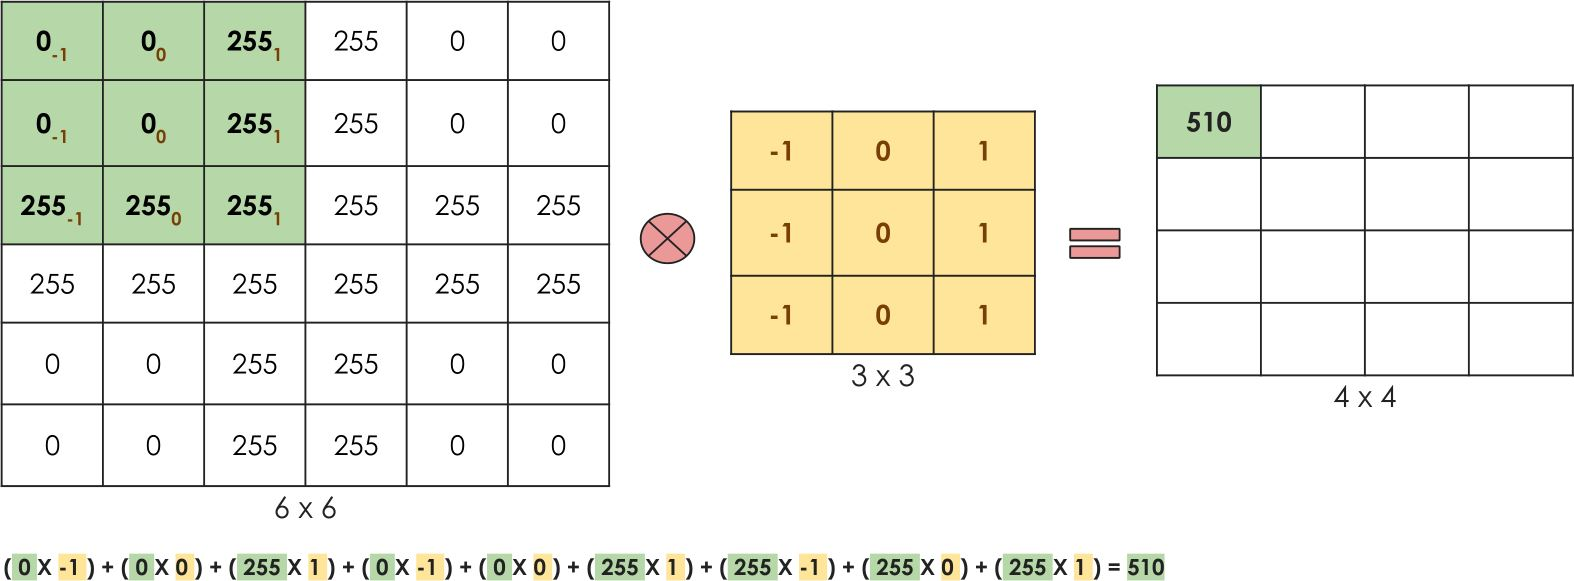
\includegraphics[height=1.5in]{convolutionoperationstep1}
				\subcaption{Step 1}
				\label{fig:convolutionoperationstep1}
			\end{minipage}

			\begin{minipage}[t]{\textwidth}
				\centering
				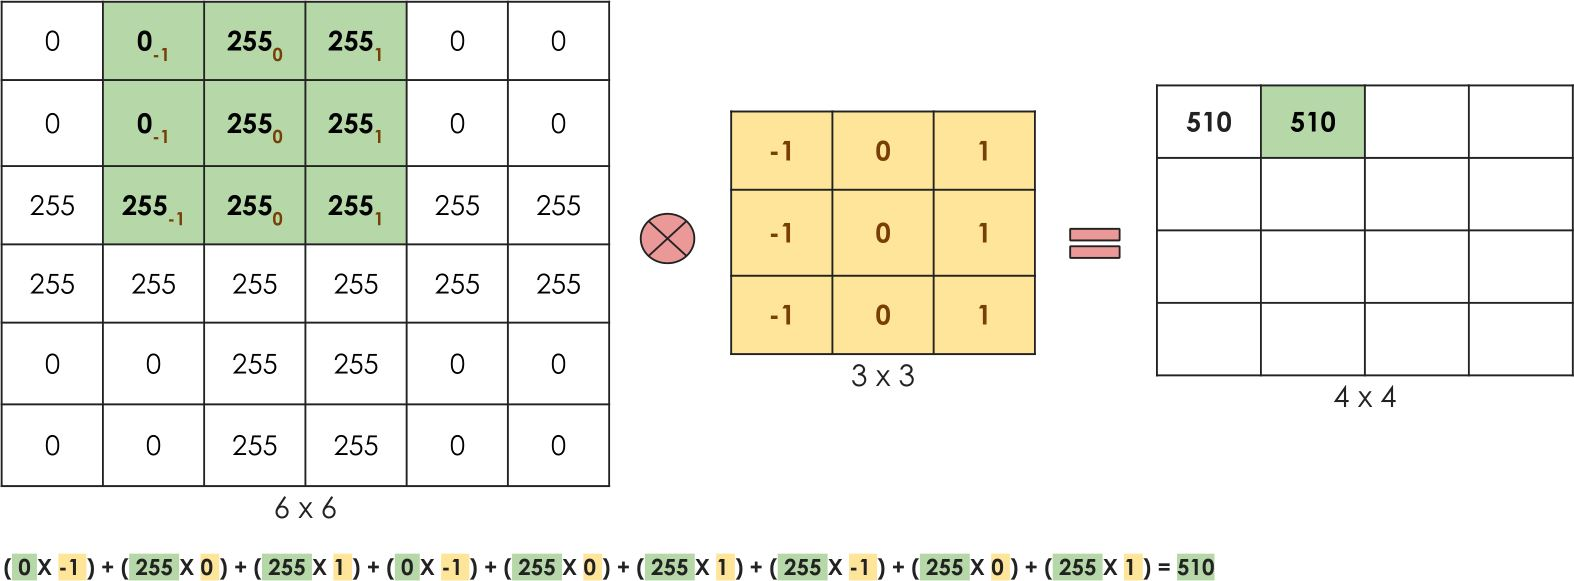
\includegraphics[height=1.5in]{convolutionoperationstep2}
				\subcaption{Step 2}
				\label{fig:convolutionoperationstep2}
			\end{minipage}

%			\vskip\baselineskip

			\begin{minipage}[t]{\textwidth}
				\centering
				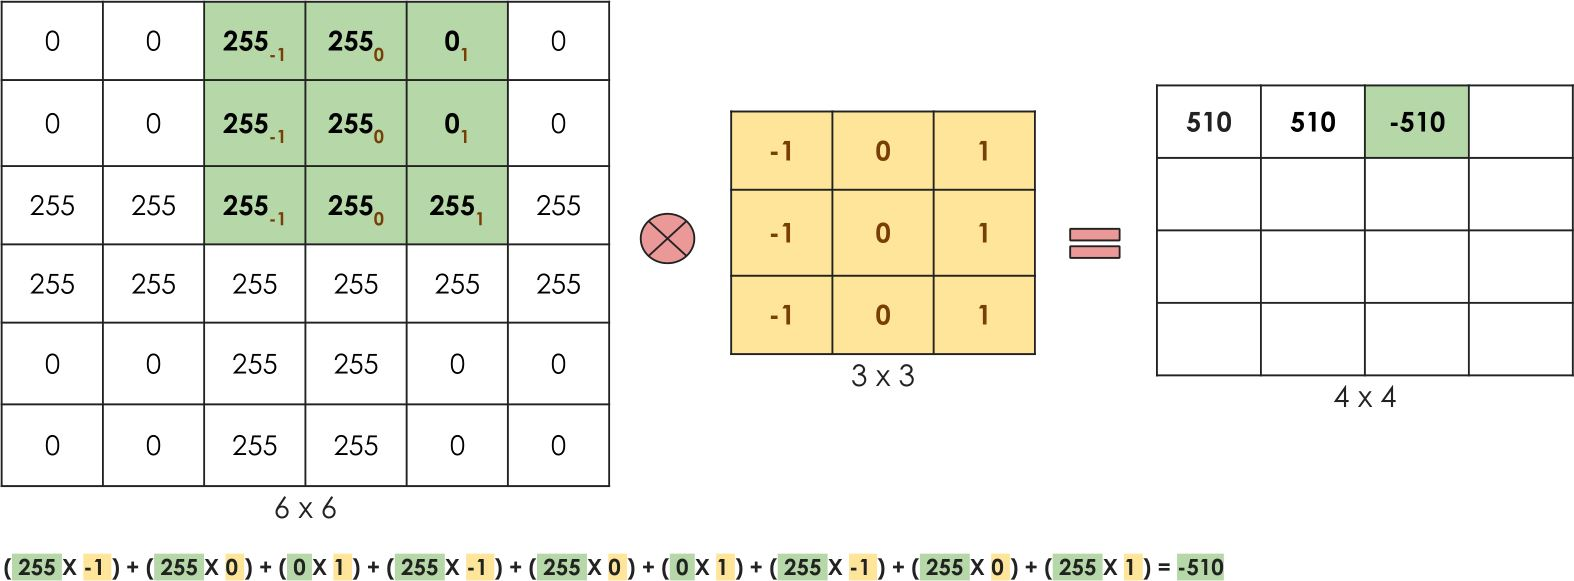
\includegraphics[height=1.5in]{convolutionoperationstep3}
				\subcaption{Step 3}
				\label{fig:convolutionoperationstep3}
			\end{minipage}

		\end{minipage}
		\caption{}
		\label{fig:convolutionoperationsteps}
	\end{figure}

	\begin{figure}[tbp]

		\begin{minipage}[t]{\textwidth}

			\begin{minipage}[t]{\textwidth}
				\centering
				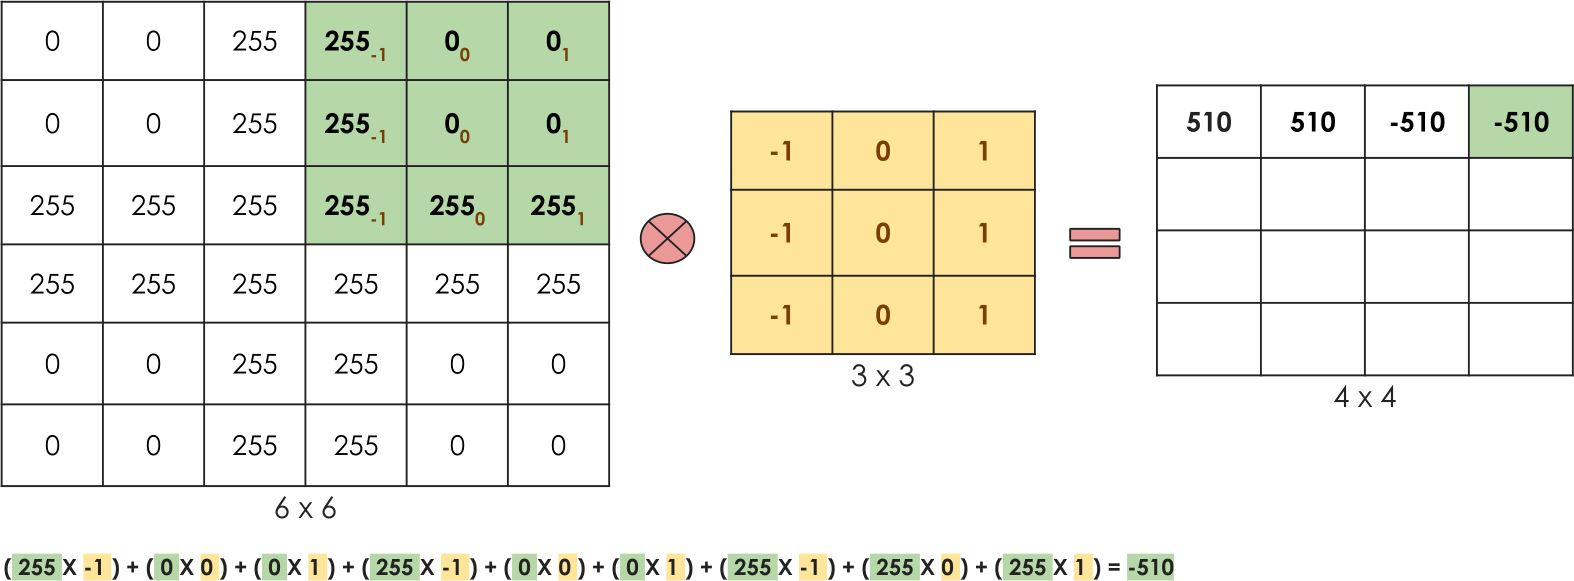
\includegraphics[height=1.5in]{convolutionoperationstep4}
				\subcaption{Step 4}
				\label{fig:convolutionoperationstep4}
			\end{minipage}

			\begin{minipage}[t]{\textwidth}
				\centering
				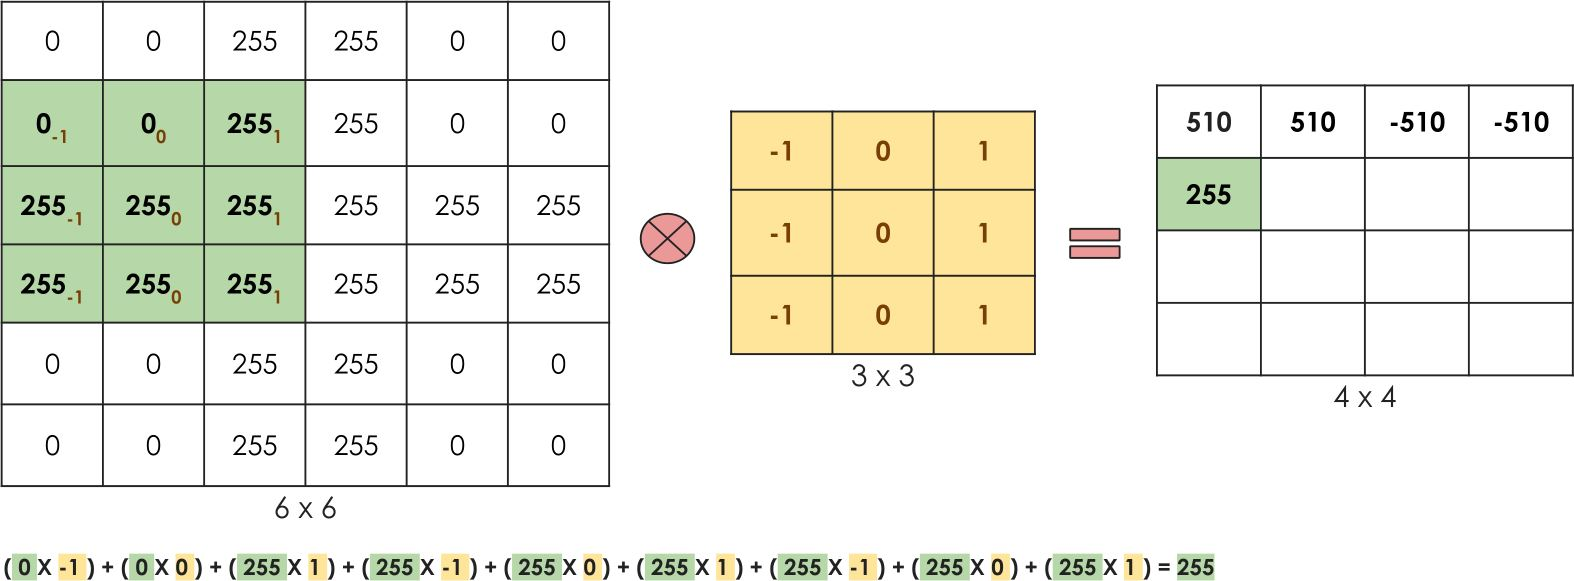
\includegraphics[height=1.5in]{convolutionoperationstep5}
				\subcaption{Step 4}
				\label{fig:convolutionoperationstep5}
			\end{minipage}

			\begin{minipage}[t]{\textwidth}
				\centering
				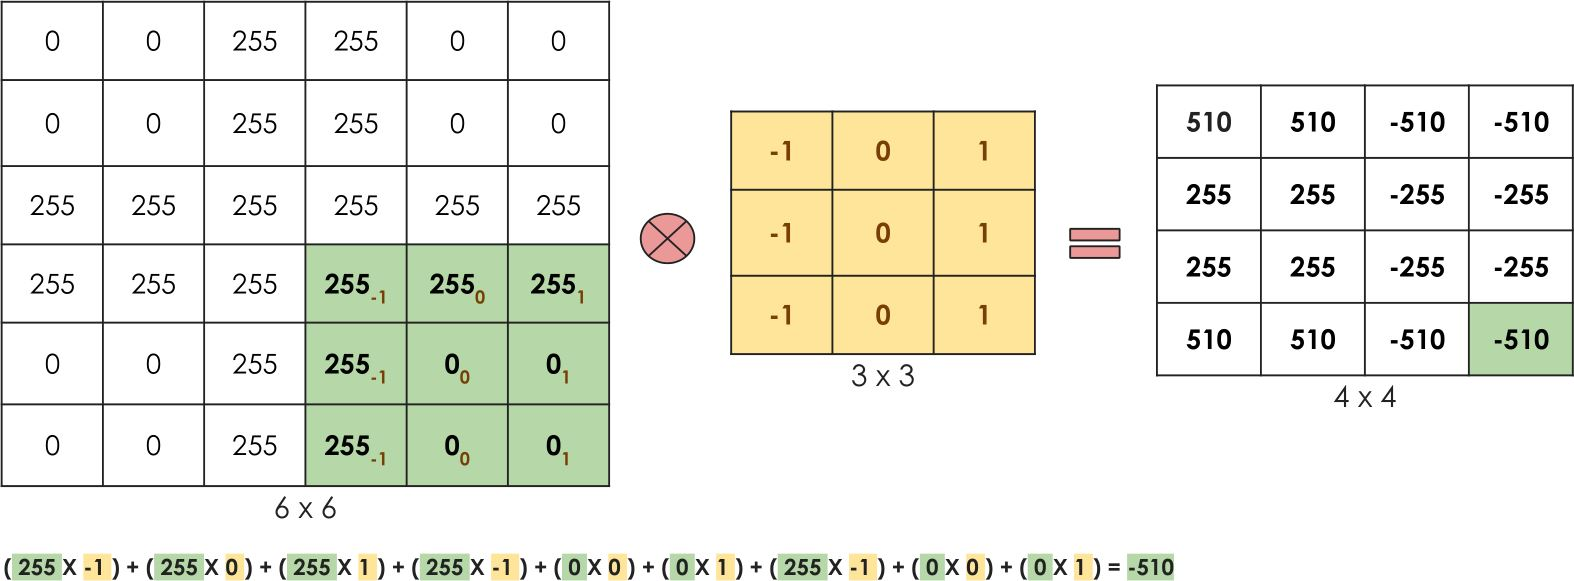
\includegraphics[height=1.5in]{convolutionoperationstep6}
				\subcaption{Step 4}
				\label{fig:convolutionoperationstep6}
			\end{minipage}

		\end{minipage}
		\caption{}
		\label{fig:convolutionoperationsteps}
	\end{figure}

	\subsection{Intuition behind Convolutions}

	\begin{bulletedlist}
		\item Convolutions can be used for various kinds of feature extraction tasks, depending only on the pixel pattern of the filter.
		\item The convolution filter used in the previous example, for instance, has a vertical pattern of -1s, 0s and 1s.  It is also known in the industry as the Prewitt Filter.
		\item The above convolution filter would be considered a type of vertical edge detector, capable of identifying vertical edges in the image.
		\item The reason for this is due to the nature of the convolution operation, which uses a sum of element-wise products. The  implication of that is those regions of the image which have similar vertical patterns to those of the filter, get amplified in
the element-wise product, and hence in the output matrix.
		\item In other words, convolution filters are adept at identifying those regions of the image which have pixel patterns that match the pixel pattern of the filter itself.
		\item That is why the above filter would be considered a type of vertical edge detector.  It has a vertical pattern of pixels (-1s, 0s and 1s) which represent a left-to-right increasing gradient.  Any regions in the input image that have a similar pattern to this would be identified by this filter, and amplified numerically with a higher output value for those regions.
		\item One other point of consideration is that filters with odd-valued dimensions (such as 3 x 3 Filters) are preferred, due to the presence of a central pixel.
		\item 
		\item 
	\end{bulletedlist}


	\subsection{Filters and Kernels}
	\begin{bulletedlist}
		\item Convolution filters can hence be used for various image manipulation tasks, such as edge detection, sharpening or blurring.
		\item As an example, let us discuss three convolution filters which have gained popularity over the years:
		\begin{bulletedlist}
			\item The Prewitt filter
			\item The Sobel filter
			\item The Laplacian filter
		\end{bulletedlist}
	\end{bulletedlist}

	\subsubsection{The Prewitt Filter}
	\begin{bulletedlist}
		\item The Prewitt filter (named after Judith M.S. Prewitt) has mostly been used in research for detecting horizontal and vertical edges in an image.
		\item This filter has three properties:
		\begin{bulletedlist}
			\item The sum of the elements in the filter is zero.
			\item The elements present in the filter should have opposite signs.
			\item The higher the magnitude of the positive and negative numbers, the higher the chances of detecting an edge.
		\end{bulletedlist}
		\item There are actually two variations of the filter, for detecting edges in both the horizontal and the vertical
directions.
	\end{bulletedlist}

	\begin{figure}[h]
		\centering
		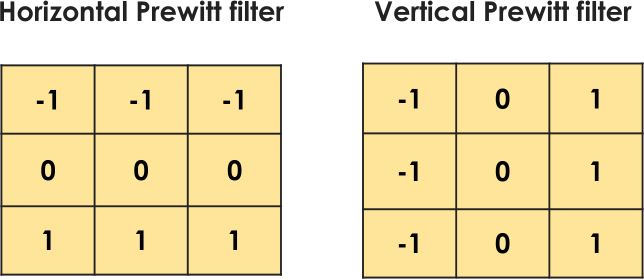
\includegraphics[height=1.2in]{prewittfilter}
		\caption{}
		\label{fig:prewittfilter}
	\end{figure}
	\begin{figure}[h]
		\centering
		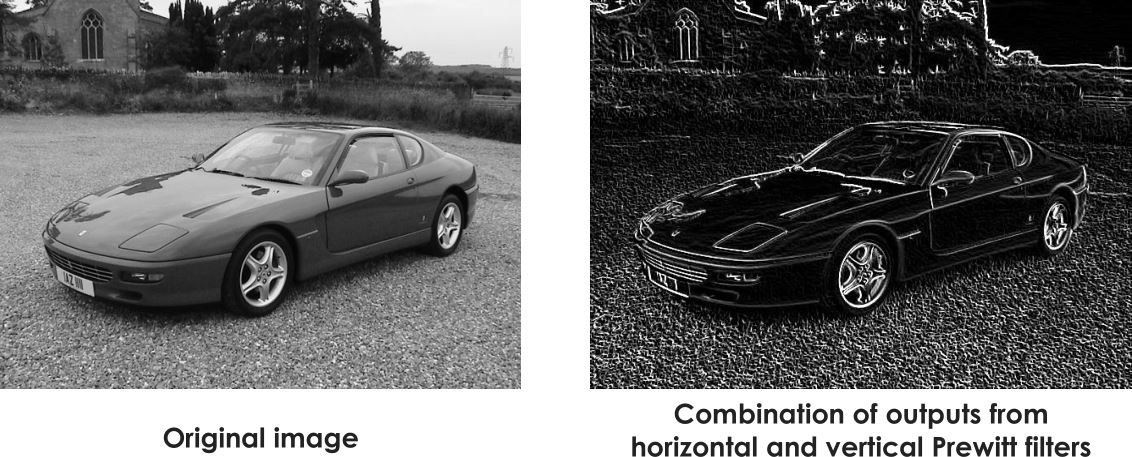
\includegraphics[height=1.75in]{prewittfilterexample}
		\caption{}
		\label{fig:prewittfilterexample}
	\end{figure}






CNN-Filters, Padding, Strides, and Pooling. 